\documentclass[11pt]{report}

\usepackage{stan-talks}

\begin{document}
\sf%
\mbox{ }
\\[12pt]
\spc{\LARGE\bfseries \color{MidnightBlue}{Taking Uncertainty Seriously}}
\\[4pt]
\spc{\large {for calibrated forecasting and decision making}}
\\[36pt]
\noindent
\spc{\Large\bfseries \color{MidnightBlue}{Bob Carpenter}}
\\[2pt]
\spc{Columbia University}
\vfill
\noindent
\spc{\small October 2019} \hfill
\hfill

\includegraphics[width=0.3in]{img/new-logo.png}

\mypart{}{Motivation}

\sld{Scientists}
\begin{itemize}
\item want to understand the world,
\item bring mechanistic theories,
\item bring data in the form of measurements, and
\item need to make predictions and evaluate theories.
\end{itemize}

\sld{Policymakers}
\begin{itemize}
\item control the social world,
\item bring hypotheses about interventions,
\item bring data in the form of measurements, and
\item need to make decisions and evaluate results.
\end{itemize}

\sld{Uncertainty}
\begin{itemize}
\item permeates science and decision making
\item in the form of
\begin{subitemize}
\item sampling uncertainty,
\item measurement uncertainty, and
\item modeling uncertainty.
\end{subitemize}
\item The alternative to good statistics is
\begin{subitemize}
\item not no statistics,
\item but bad statistics.
\end{subitemize}
\end{itemize}

\sld{Probability \& Statistics}
\begin{itemize}
\item Probability uses math to quantify uncertainty.
\item Bayesian statistics applies probability theory to
\begin{subitemize}
\item data analysis,
\item prediction \& forecasting,
\item decision theory, and
\item model evaluation.
\end{subitemize}
\end{itemize}

\sld{This talk}
\begin{itemize}
\item How to combine data, theory, and probability to
\begin{subitemize}
\item make calibrated predictions,
\item optimal decisions under uncertainty, and
\item solve the replication crisis.
\end{subitemize}
\item Plus a summary of my current work on
\begin{subitemize}
\item algorithms,
\item methodology, and
\item applications.
\end{subitemize}
\end{itemize}

\mypart{}{Bayesian Inference}

\sld{Notation}
\begin{itemize}
\item Variables
\begin{subitemize}
\item $y$ : data (observed)
\item $\theta$ : parameters (unknown)
\end{subitemize}
\item Probability functions
\begin{subitemize}
\item $p(y, \theta)$ : joint density
\item $p(y \mid \theta)$ : sampling density
{\footnotesize \hfill (likelihood as fun of $\theta$)}
\item $p(\theta)$ : prior (parameter marginal)
\item $p(\theta \mid y)$ : posterior
\item $p(y)$ : evidence (data marginal)
\end{subitemize}
\end{itemize}

\sld{Bayesian inversion}
{\footnotesize
\begin{eqnarray*}
p(\theta \mid y) & = & \frac{p(y, \theta)}{p(y)}
\\[4pt]
& = & \frac{p(y \mid \theta) \cdot p(\theta)}{p(y)}
\\[4pt]
& = & \frac{p(y \mid \theta) \cdot p(\theta)}{\int_{\Theta} p(y, \theta) \, \textrm{d}\theta}
\\[4pt]
& = & \frac{p(y \mid \theta) \cdot p(\theta)}{\int_{\Theta} p(y \mid \theta) \cdot p(\theta) \, \textrm{d}\theta}
\\[10pt]
& \propto &
p(y \mid \theta) \cdot p(\theta).
\end{eqnarray*}
\begin{subitemize}
\item posterior proportional to likelihood times prior
\end{subitemize}
}

\sld{Estimators, predictions, and events}
\begin{itemize}
\item Parameter estimate
{\footnotesize $$
\hat{\theta}
\ = \ \mathbb{E}[\theta \mid y]
\ = \ \textstyle
\int_{\Theta} \theta \cdot p(\theta \mid y) \, \textrm{d}\theta.
$$}
\item Event probability ($A \subseteq \Theta$, \ \ {\footnotesize e.g., $A = \{ \theta \in \Theta : \theta > 0\}$})
{\footnotesize $$
\textrm{Pr}[A \mid y]
\ = \ \mathbb{E}[\textrm{I}_A(\theta) \mid y]
\ = \ \textstyle
\int_{\Theta} \textrm{I}_A(\theta) \cdot p(\theta \mid y)
\, \textrm{d}\theta.
$$}
\item Predictive inference
{\footnotesize $$
p(\tilde{y} \mid y)
\ = \ \mathbb{E}[p(\tilde{y} \mid \theta) \mid y]
\ = \ \textstyle
\int_{\Theta} p(\tilde{y} \mid \theta) \cdot p(\theta \mid y)
\, \textrm{d} \theta.
$$}
\end{itemize}

\sld{(Markov chain) Monte Carlo}
\begin{subitemize}
\item Given sample $\theta^{(1)}, \ldots, \theta^{(M)} \sim p(\theta \mid y).$
\item General plug-in expectation calculations,
\begin{eqnarray*}
\mathbb{E}[f(\theta) \mid y]
& = &
\int_{\Theta} \, f(\theta) \cdot p(\theta \mid y) \, \textrm{d}\theta
\\[8pt]
& = &
\lim_{M \rightarrow \infty} \,
\frac{1}{M} \, \sum_{m=1}^M \, f\!\left(\theta^{(m)}\right)
\\[8pt]
& \approx &
\frac{1}{M} \, \sum_{m=1}^M \, f\!\left(\theta^{(m)}\right).
\end{eqnarray*}
\item (MCMC) central limit theorem: finite approx error $\propto \frac{\displaystyle 1}{\displaystyle \sqrt{M}}$
\end{subitemize}

\mypart{}{Examples}

\sld{Birth ratio \hfill {\Large (Laplace, 1781)}}
\begin{itemize}
\item Live births in Paris, 1745--1770
\begin{subitemize}
\item $y = 251,527$ male, $N = 493,472$ total
\end{subitemize}
\item Sampling:
$p(y \mid N, \theta)
 = \textrm{binomial}(y \mid N, \theta).$
\item Prior:
$p(\theta)
 = \textrm{uniform}(\theta \mid 0, 1)$
\item Posterior:
$p(\theta \mid y)
 = \textrm{beta}(\theta \mid 1 + y, \ 1 + N - y).$
\item {\small $\textrm{Pr}[\theta \in (0.508, 0.512)] = 0.99$}
\hfill {\footnotesize (estimated male birth rate)}
\item {\small $\textrm{Pr}[\theta > 0.5] \approx 1 - 10^{-42}$}
\hfill {\footnotesize (``morally certain'' more boys)}
\end{itemize}

\sld{Birth ratio in Stan}
\begin{stancode}
transformed data {
  int y = 251527;  int N = 493472;
}
parameters {
  real<lower=0, upper=1> theta;
}
model {
  y ~ binomial(N, theta);
}
generated quantities {
  int<lower=0, upper=1> theta_gt_half = (theta > 0.5);
  int<lower = 0> y_sim = binomial_rng(100, theta);
}
\end{stancode}

\sld{And the answer is...}
%
\begin{codein}
> fit <- stan("laplace.stan")
> print(fit, probs=c(0.005, 0.995), digits=3)
\end{codein}
\begin{codeout}
                     mean se_mean   0.5%   99.5%
theta               0.510   0.000  0.508   0.512
theta_gt_half       1.000     NaN  1.000   1.000
y_sim              50.902   0.081 38.000  64.000
\end{codeout}
%
\begin{subitemize}
\item estimate $\hat{\theta}$ is posterior sample mean for $\theta$;
\item 99\% interval for $\theta$ estimated by sample quantiles
\item $\textrm{Pr}[\theta > 0.5]$ estimated by sample mean of indicator
\item {\texttt y\_sim} estimated forecast for next 100 births
\end{subitemize}

\sld{Population Dynamics \hfill {\large (Volterra 1926)}}
\begin{itemize}
\item populations at $t$ of prey $u(t)$ \& predator $v(t)$
\item Volterra's mechanistic model
$$
\frac{\textrm{d}}{\textrm{d}t}u = (\alpha - \beta \cdot v) \cdot u
\qquad
\frac{\textrm{d}}{\textrm{d}t}v = (-\gamma + \delta \cdot u) \cdot v
$$
\vspace*{-12pt}
\begin{subitemize}
\item $\alpha$: prey growth rate;  \ $\beta$: predation shrinkage
\item $\gamma$: predator shrinkage; \ $\delta$: predation growth
\end{subitemize}
\end{itemize}

\sld{Analytic solutions \hfill {\large (Volterra 1926)}}

\begin{center}
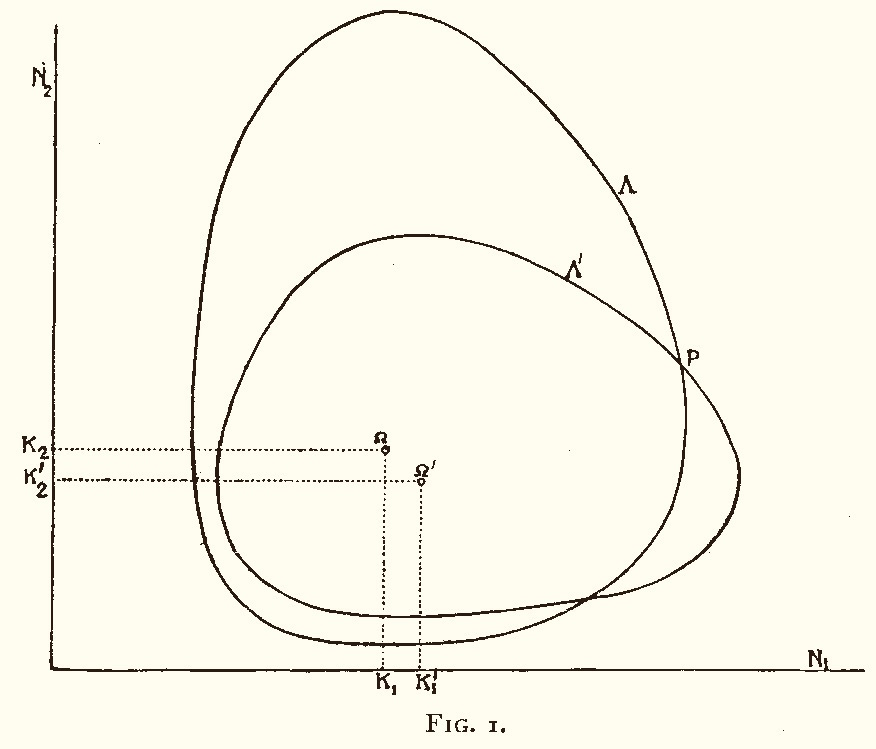
\includegraphics[width=0.6\textwidth]{img/volterra-solutions.jpg}
\end{center}

\sld{Measurement error model}
\begin{itemize}
\item $u, v$ are observed
\item $\hat{u}, \hat{v}$ predicted by mechanistic model
\item Independent error proportional to population size
\begin{subitemize}
\item $u_t \sim \textrm{lognormal}(\hat{u}_t, \sigma_1)$
\item $v_t \sim \textrm{lognormal}(\hat{v}_t, \sigma_2)$
\end{subitemize}
\item Weakly informative priors inform scale
\begin{subitemize}
\item $\alpha, \gamma \sim \textrm{normal}(1, 0.5)$; \ \ \
$\beta, \delta \sim \textrm{normal}(0.05, 0.05)$
\item $\sigma_1, \sigma_2 \sim \textrm{lognormal}(-1, 1)$
\end{subitemize}
\end{itemize}

\sld{Hudson's Bay Co.\ Pelts \hfill {\large (Hewitt 1921)}}
\begin{center}
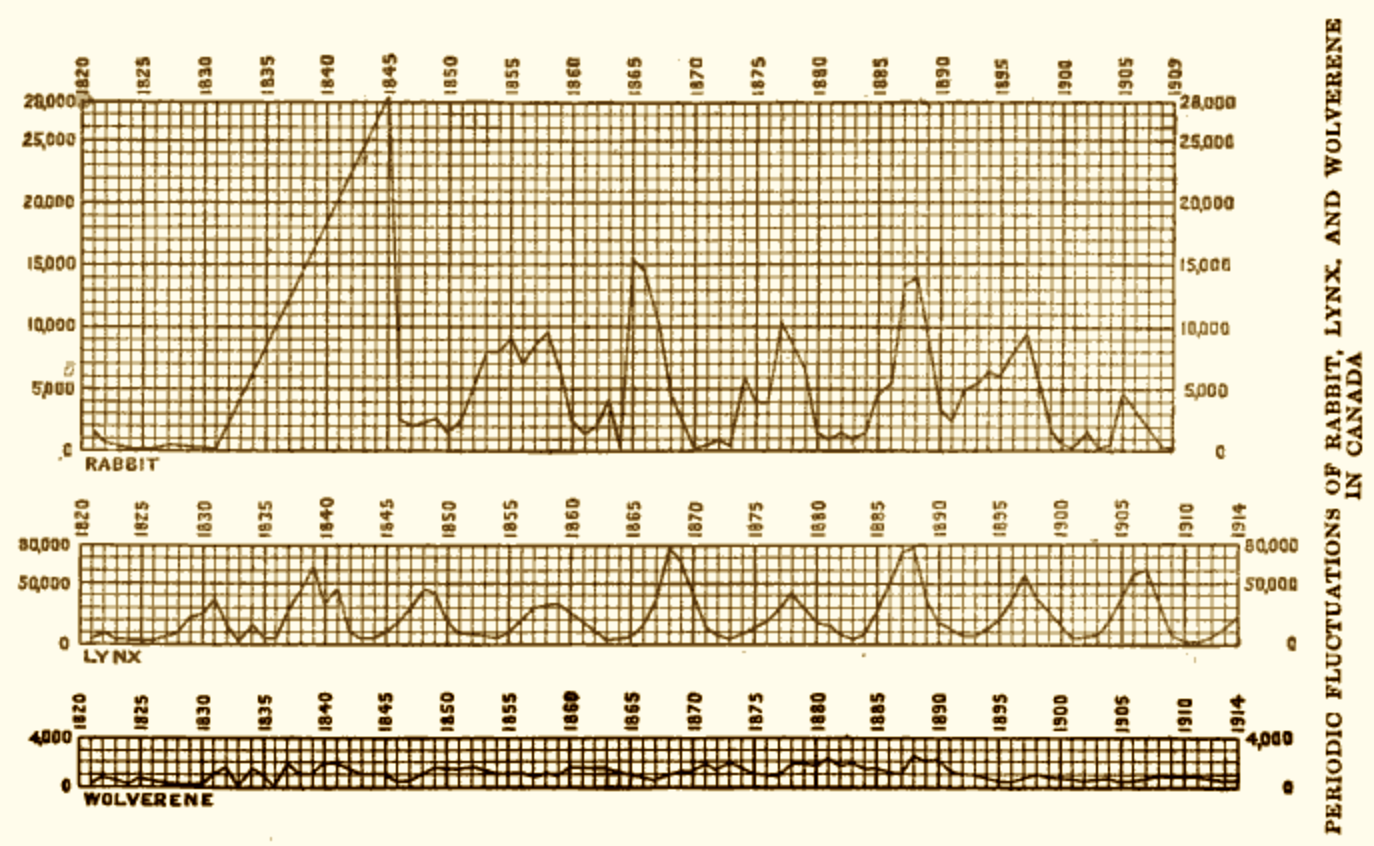
\includegraphics[width=0.9\textwidth]{img/hudons-bay-data.png}
\end{center}

\sld{Munged and plotted}
\begin{center}
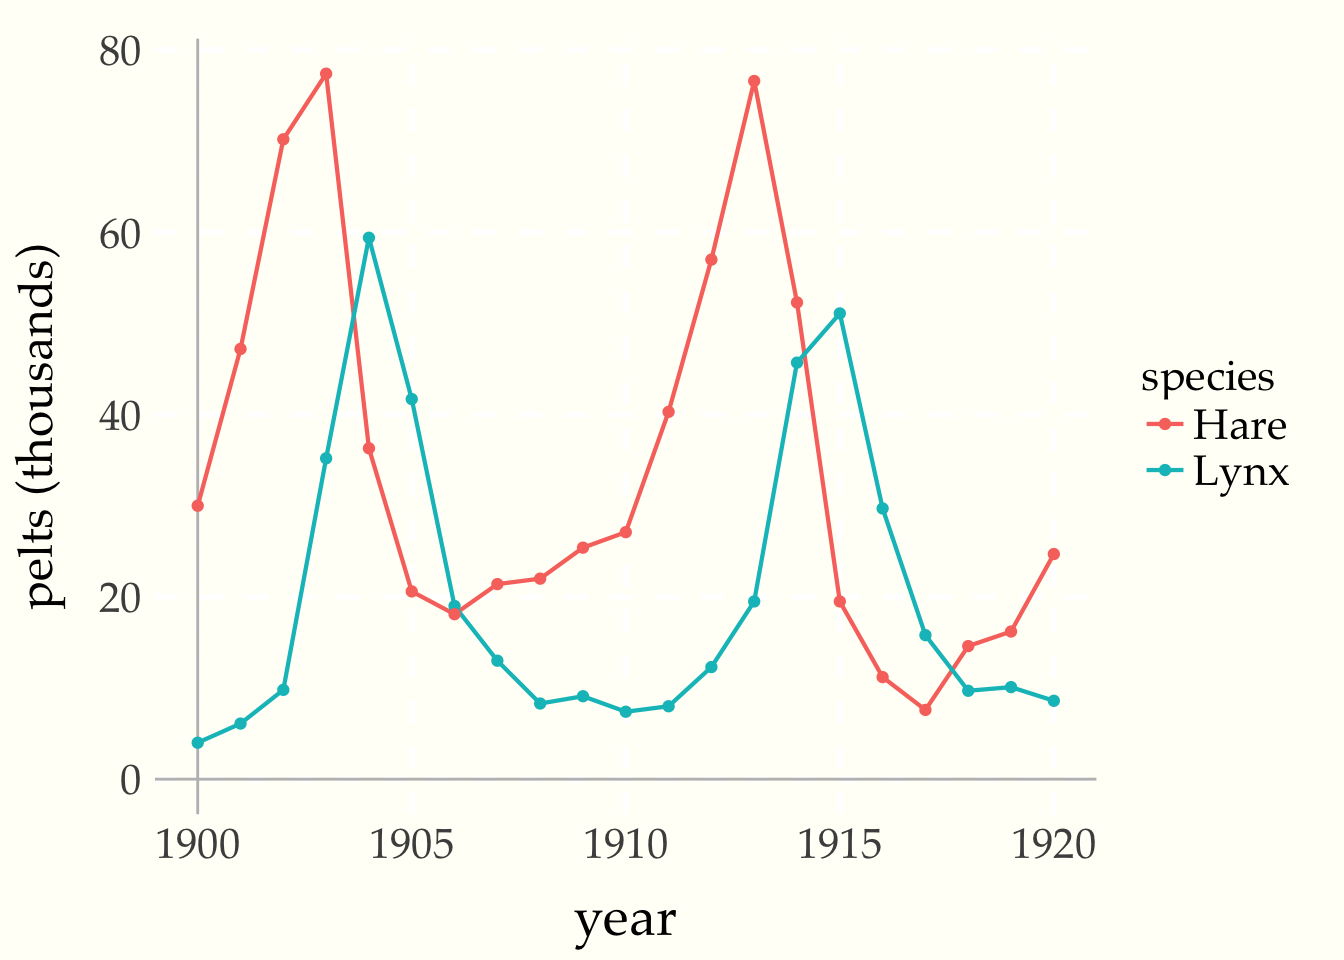
\includegraphics[width=0.45\textwidth]{img/lynx-hares-1.png}~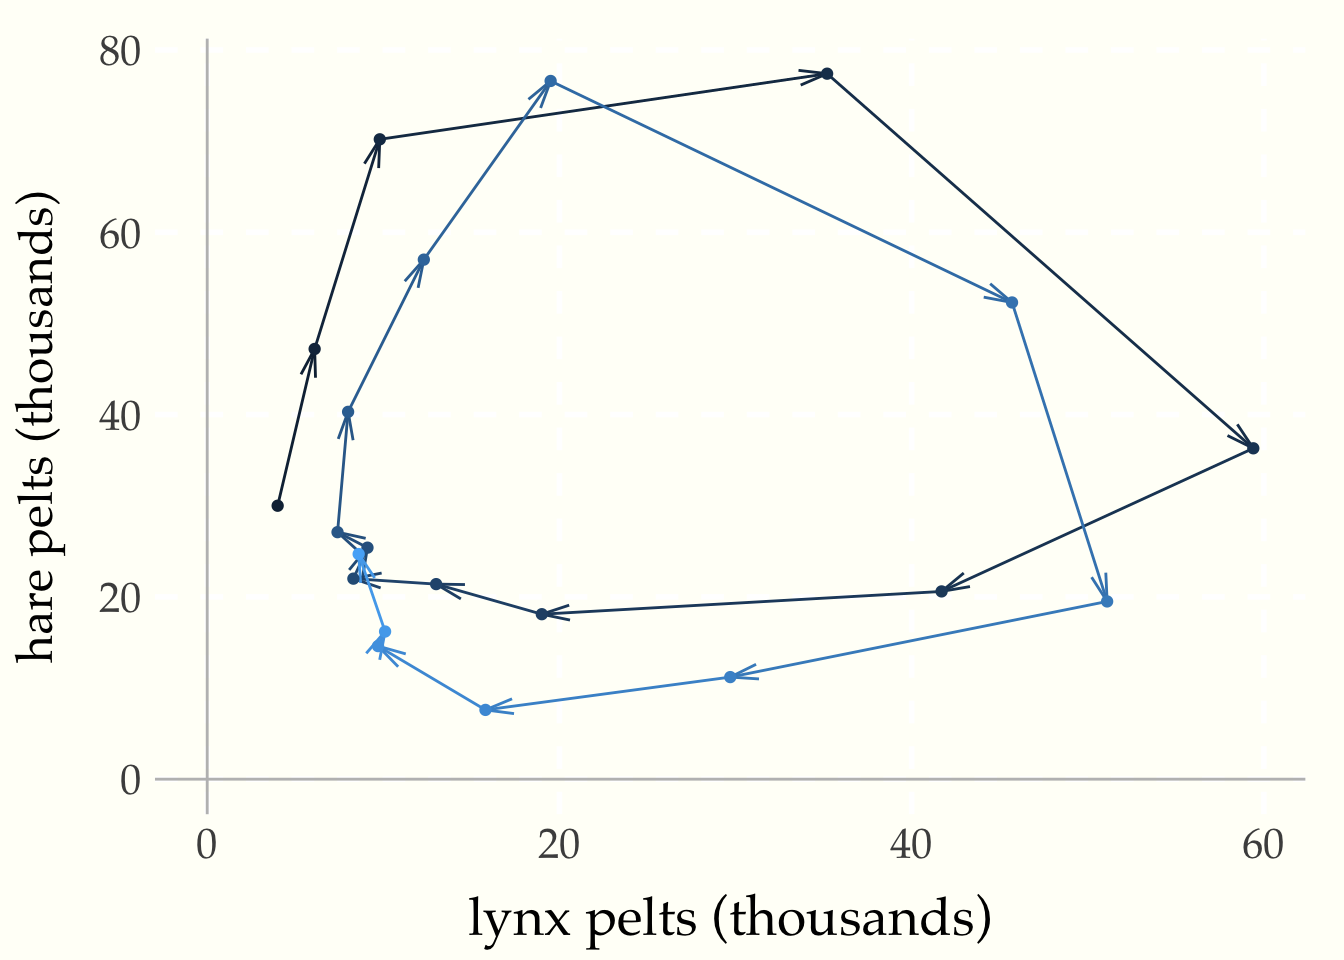
\includegraphics[width=0.45\textwidth]{img/lynx-hares-2.png}
\end{center}
\begin{itemize}
\item {\it left)} pelts vs. time \hfill
{\it right)} hare vs. lynx pelts
\\
(line per species) \hfill (over time)
\end{itemize}

\sld{Stan dynamics \& meas.\ error}
\begin{stancode}
real[] dz_dt(real t, real[] uv, real[] theta,
             real[] theta, real[] x_r, int[] x_i) {
  return { (theta[1] - theta[2] * uv[2]) * uv[1],
           (-theta[3] + theta[4] * uv[1]) * uv[2] };
}
...
real z[T, 2]
  = integrate_ode(dz_dt, z0, t0, sol_ts[1:T], theta,
                  rep_array(0.0, 0), rep_array(0, 0));
...
y[1:T, 1] ~ lognormal(z[1:T, 1], sigma_u);
y[1:T, 2] ~ lognormal(z[1:T, 2], sigma_v);
\end{stancode}

\sld{Measurements \& predictions}
\begin{center}
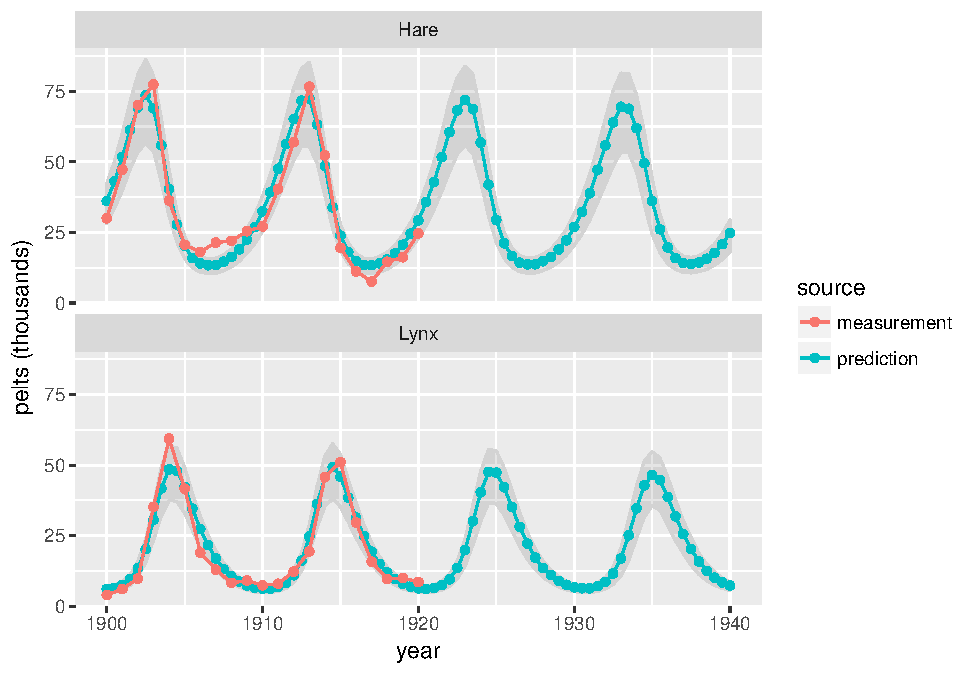
\includegraphics[width=0.8\textwidth]{img/lotka-volterra-posterior.pdf}
\end{center}

\sld{As evolving over time}
\begin{center}
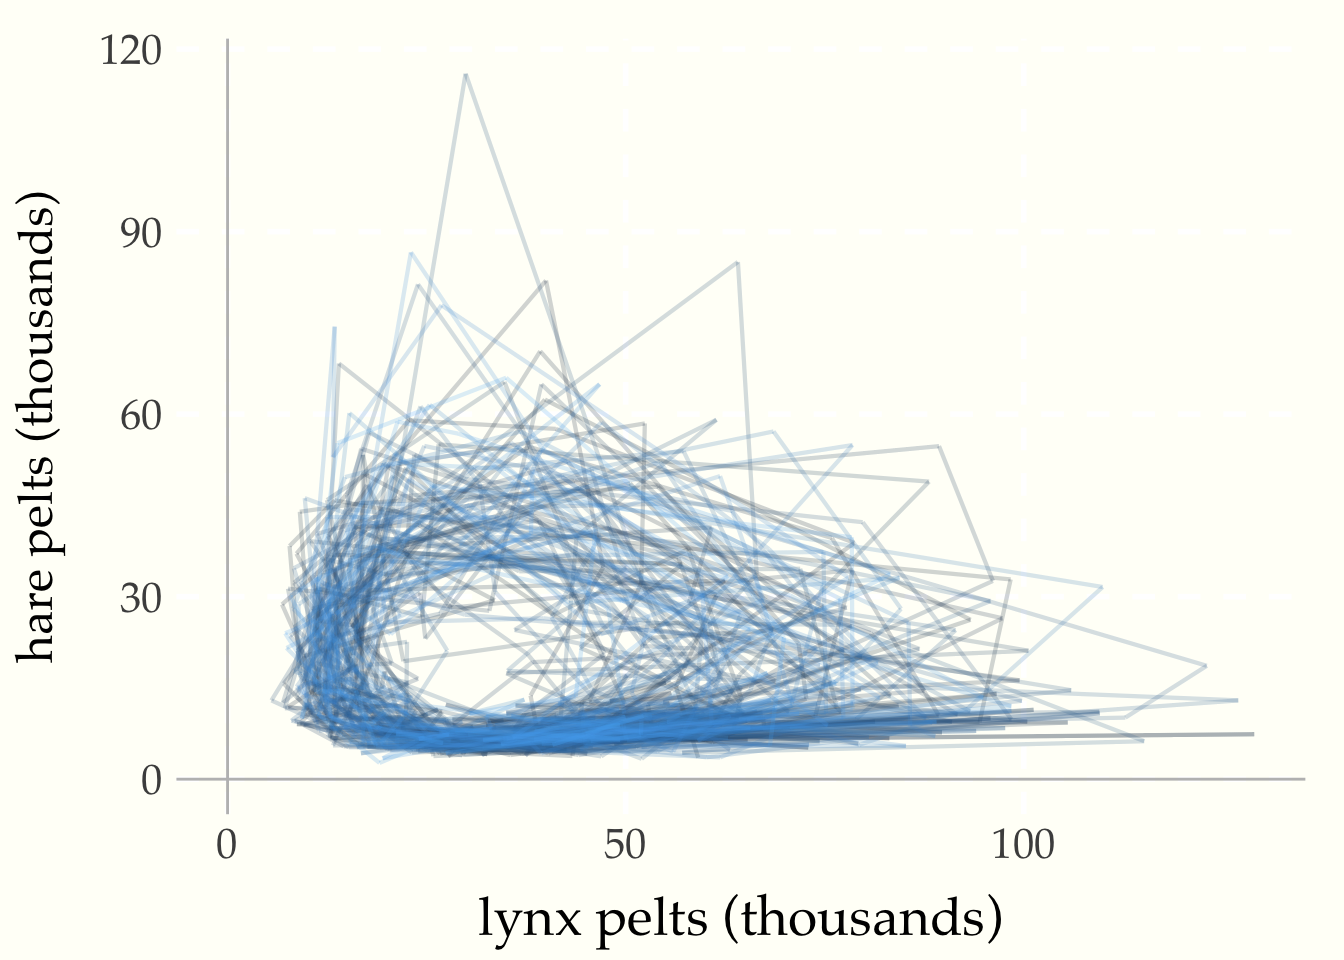
\includegraphics[width=0.8\textwidth]{img/lotka-volterra-posterior-time.png}
\end{center}


\mypart{}{Projects}

\sld{Methodology}
\begin{itemize}
\item Bayes vs. all contenders for proper scoring evaluation
\item Model evaluation and comparison with uncertain crowdsourced data
\item Partial pooling to estimate performance with multiple comparisons
\end{itemize}

\sld{Algorithms}
\begin{itemize}
\item Asynchronous parallel adapation of MCMC
\item Sequential HMC for filtering (i.e., online learning)
\item Matrix automatic differentiation
\item Parallel automatic differentiation
\item Higher-order automatic differentiation
\end{itemize}

\sld{Applications}
\begin{itemize}
\item Arctic soil-carbon response to environmental change
\begin{subitemize}
\item Kathe Todd-Brown (U.\ Florida, env. engnr)
\item Sean Schaeffer (U.\ Tennessee, ag.)
\end{subitemize}
\item Differential expression of gene splice variants with biological replicates
\begin{subitemize}
\item Shuonan Chen (Columbia, biostats)
\item Chaolin Zhang (Columbia, genomics)
\end{subitemize}
\end{itemize}

\sld{Applications (II)}
\begin{itemize}
\item Virtual database completion for the National Election Survey
\begin{subitemize}
\item Andrew Gelman (Columbia, stats \& poli sci)
\item Steve Ansolabehere (Harvard, poli sci)
\end{subitemize}
\item Educational testing and teacher evaluation
\begin{subitemize}
\item Andrew Gelman (Columbia, stats \& poli sci)
\item Sophia Rabe-Hesketh (UC Berkeley, ed and biostats)
\end{subitemize}
\end{itemize}

\sld{Applications (III)}
\begin{itemize}
\item Equilibrium and rational decision making in auction pricing
\begin{subitemize}
\item Tom Sargent (NYU, economics)
\item Shoshanna Vasserman (Stanford, business)
\item Rachel Meager (LSE, economics)
\end{subitemize}
\item Crowdsourced training and evaluation in machine learning
\begin{subitemize}
\item Massimo Poesio (U. Essex, comp sci)
\item Becky Passonneau (Penn State, comp sci)
\end{subitemize}
\end{itemize}

\end{document}
